\section{PDES Design}

In order to create a realistic model, we decided to use two logic processors (LP). 
One LP represents an airport and the other LP represents a region controller.
An airport LP contains 9 state variables and a region controller LP contains 6 state variables.
We used 13 different event types and run Dijkstra shortest path algorithm to send an airplane along path to the destination airport.
Two limitation existed. We can not use an array. We can not use a loop. 
This is due to Backstroke doesn't handle arrays and loops in generating a reverse code.  
Figure \ref{fig:sim_flow} shows the simulation flow as seen from the perspective of a single flight.
The black circle represents an airport and the red circle represents a region controller. 
The model contains a request/response structure between two different types of LP.
This structure requires to include the sender's information when it schedules an events, so that 
the receiver LP can response back to the sender LP.
We used a message structure in ROSS, which is a wrapper of an event which allows to store data for the event. 
The straight arrow represents a time for scheduling an event and the dotted arrow indicates a delay. 


\begin{figure} [h]
\centering
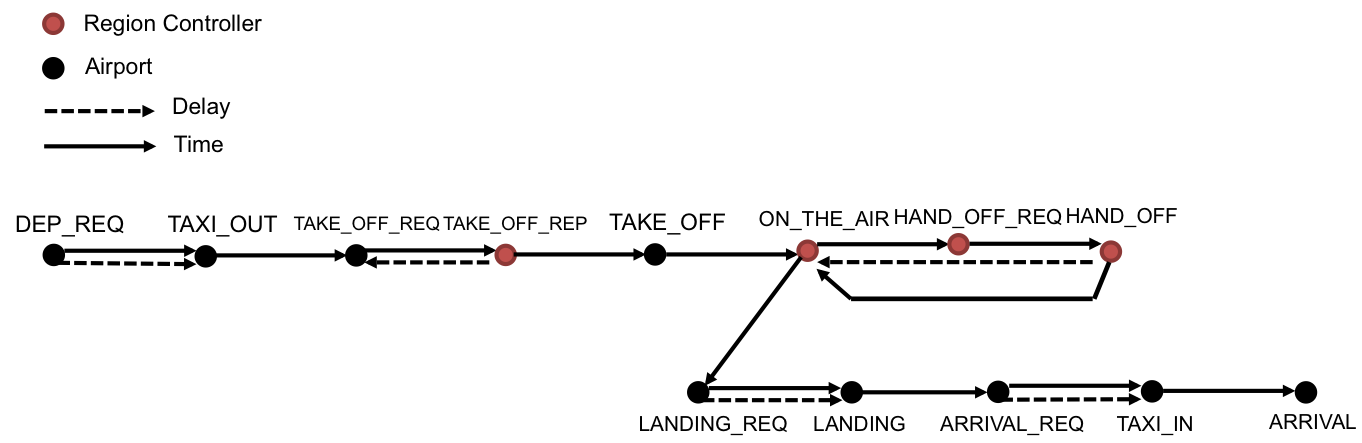
\includegraphics[width=5.2in]{/Users/chayong/Documents/project2/figs/sim_flow.png}
\caption{Air Traffic Simulation Flow}
\label{fig:sim_flow}
\end{figure}